\chapter{Recherche}

In diesem Kapitel wird erklärt was BPMN ist, es werden die Rahmenbedingungen umrissen und die verschiedenen Programme analysiert welche für die Umsetzung in Frage kommen.

\section{BPMN}
BPMN steht für Business Process Model and Notation. Dabei handelt es sich um eine genormte Visualisierung für Business Processes. Entwickelt wurde der Standart im Jahre 2001 durch die Firma IBM.

\subsection{Notation}
\label{sec:Recherche:bpmn:notation}
In diesem Abschnitt soll die grundlegenden Objekte von BPMN vorgestellt werden.

\begin{figure}[H]
	\centering
	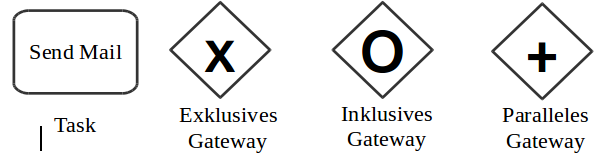
\includegraphics[width=0.6\textwidth]{images/bpmn-flow-objects.png}
	\caption{Flow Objects}
	\label{fig:recherche:bpmn:flowobjects}
\end{figure}
Der Task ist ein Schritt eines Prozesses, welcher ausgeführt wird. Dieser kann entweder durch einen Menschen oder automatisiert durchgeführt werden. Die Rauten sind Gateways. Das Exklusive (XOR) Gateway, steht für einen Entscheidung. Es kann nur ein Pfad weitergeführt werden. Deshalb heisst es exklusiv. Das Inklusive (OR) Gateway ist wie das Exklusive Gateway eine Entscheidung, es können jedoch mehrere Wege parallel ausgeführt werden. Das Paralelle (AND) Gateway führt alle Pfade parallel aus. Es kann auch dazu verwendet werden mehrere Pfade zu synchronisieren und als einzelner Weg weiterzuführen.

\begin{figure}[H]
	\centering
	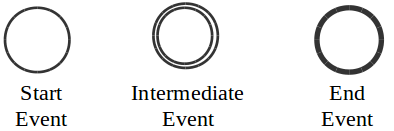
\includegraphics[width=0.4\textwidth]{images/bpmn-flow-objects2.png}
	\caption{Events}
	\label{fig:recherche:bpmn:events}
\end{figure}
Ein Event beschreibt, wenn etwas während eines Prozesses passiert. Oben aufgeführt sind die drei Grundevents. Der Start Event kennzeichnet der Beginn und der End Event das Ende eines Prozesses. Ein Intermediate Event kann irgendwo zwischen dem Start und dem Ende eines Prozesses stehen. Es gibt diverse Ausprägungen von Events, welche mit Icons in den Kreisen gekennzeichnet werden. Zum Beispiel ein Mail Event, Timer Event, Error Event, Cancel Event, Link Event, Signal Event und Terminate Event, um einige zu nennen.

\begin{figure}[H]
	\centering
	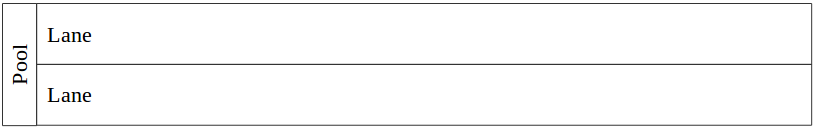
\includegraphics[width=0.8\textwidth]{images/bpmn-pool-swimlanes.png}
	\caption{Pool and Swimlanes}
	\label{fig:recherche:bpmn:poolswimlanes}
\end{figure}
Ein Pool kennzeichnet einen Participant, einen Benutzer oder Benutzerrolle in einem Prozess. Swimlanes ziehen sich über den gesamten Pool und werden dazu benutzt diesen weiter zu unterteilen.

\begin{figure}[H]
	\centering
	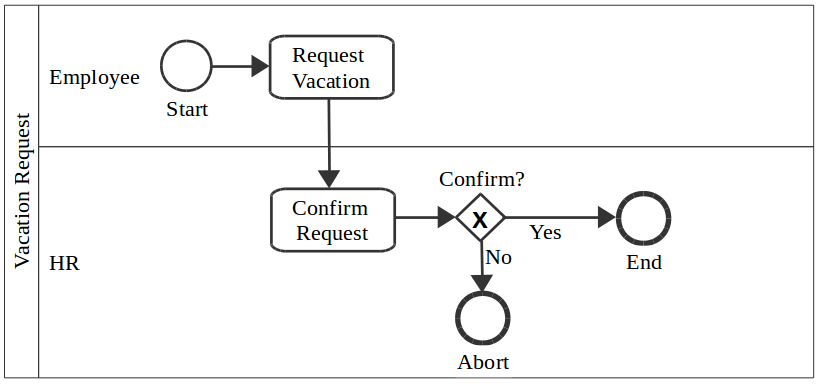
\includegraphics[width=0.8\textwidth]{images/bpmn-example.png}
	\caption{Example}
	\label{fig:recherche:bpmn:example}
\end{figure}
Dies ist eine einfaches Beispiel eines Vacation Request Prozesses. Der Arbeitnehmer startet den Prozess und stellt seine Ferienanfrage. Die Anfrage wird von der Personalabteilung weiterverwendet und entscheidet, ob die Anfrage genehmigt wird oder nicht.

\section{Rahmenbedingungen}
Zu den Rahmenbedingungen gehört die Infrastruktur der travel.ch Webseite, das Entwicklungssystem des Programmierers sowie die etablierten Prozesse der travelwindow AG, welche die Webseite travel.ch betreibt.

\subsection{Travelwindow AG Prozesse}
\label{sec:Recherche:rahmenbedingungen:prozesse}
Die Travelwindow AG ist der Betreiber der Seite travel.ch, auf welcher verschiedene Produkte gekauft werden können. Flüge, Hotel, Badeferien, Städtereisen sowie Hotel und Flug Kombinationen. Da der Buchungsprozess für Hotel und Flug Kombinationen der längste ist, wurde entschieden dass dieser in dieser Arbeit modelliert werden soll. 

\begin{figure}[H]
	\centering
	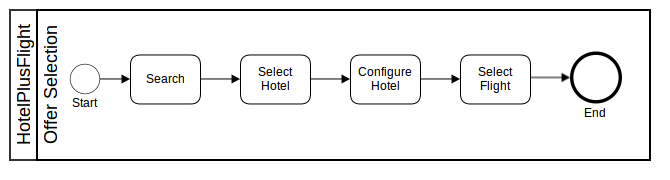
\includegraphics[width=0.8\textwidth]{images/hotelplusflight.png}
	\caption{Hotel plus Flight BPMN Model auf travel.ch}
	\label{fig:recherche:rahmenbedingungen:hotelplusflight}
\end{figure}
Der Prozess der Hotel und Flug Suche auf der travel.ch Webseite ist linear. Nach einer Produktsuche muss der Kunde ein Hotel wählen, welches er danach noch weiter Konfigurieren kann. Dabei kann er andere Zimmer- und Verpflegungstypen wählen. Zum Schluss erhält er eine Auswahl von Flügen bevor der Prozess mit einem End Event terminiert.

\subsection{Travelwindow AG API}
\label{sec:Recherche:rahmenbedingungen:api}
Travel.ch besteht aus einer Webseite und einer \Gls{glos:api}. Für die Ausführung der Prozesse via BPMN muss die API angesprochen werden. Diese liefert daten in \Gls{glos:json} aus. Programme für das ausführen des travel.ch BPMN Prozesses muss demnach den Austausch von Daten über eine \Gls{glos:api} mittels \Gls{glos:json} ermöglichen.

\subsection{Betriebsystem}
Die travel.ch Webseite wird über eine \Gls{glos:api} betrieben, welche mittels eines BPMN Programmes abgefragt werden soll. Diese \Gls{glos:api} ist nur vom Firmennetzwerk aus erreichbar. In der Firma sind nur Rechner mit dem Windows Betriebsystem im Einsatz.

Das Entwicklungssystem des Programmierers ist eine Linux Mint Computer. Dabei handelt es sich um ein Unix basiertes Betriebsystem.

Es ist demnach zwingend Notwendig, dass das BPMN Programm auf Windows, sowie auf Unix basierten Betriebssystemen läuft.

\section{travel.ch Webseite}
\label{sec:recherche:travelch}
Da die Webseite der Travelwindow AG in BPMN dargestellt werden soll, wird nachfolgend das Interface der Seite aufgezeigt.
\begin{figure}[H]
	\centering
	
\includegraphics[width=0.8\textwidth]{images/travel-search.png}
	\caption{Hotel und Flug suche auf travel.ch}
	\label{fig:recherche:travelch:search}
\end{figure}
Das Reiseziel definiert das Ziel des Fluges und wo das Hotel gesucht wird. Als Reisedaten gibt es eine exakte und eine flexible Suche. Bei einer flexiblen Suche gibt man einen Reisezeitraum (z.B. 6 Monate) an und definiert, wie lange die Reise sein soll (z.B. 7 Tage). Dann kann man das günstigste Objekt in diesem Zeitraum aussuchen. Bei der exakten Suche gibt man das Hinreise- und Rückreisedatum genau an.
Im Feld Personen/Zimmer kann man Räume definieren und wie viele Passagiere in diesen übernachten. Es wird zwischen Erwachsenen und Kinder unterschieden, da bei den Kindern zusätzlich das Geburtsdatum angegeben werden muss. Der Abflug ab gibt an, ab wo man fliegen möchte. Dies ist eine fixe Liste mit folgenden Flughäfen:
\begin{itemize}
\item Basel-Mülhausen
\item Bern-Belp
\item Genève-Cointrin
\item Zürich
\item Friedrichshafen
\item Mailand-Malpensa
\end{itemize}

\begin{figure}[H]
	\centering
	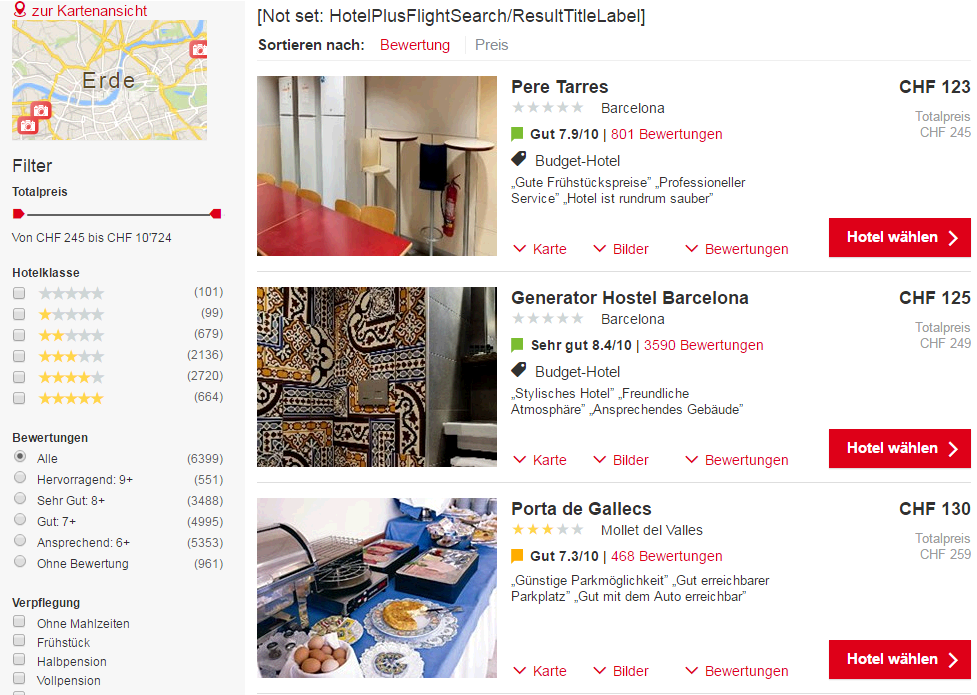
\includegraphics[width=0.8\textwidth]{images/travel-results.png}
	\caption{Hotel und Flug Hotelresultate auf travel.ch}
	\label{fig:recherche:travelch:results}
\end{figure}
Bei den Hotelresultaten gibt es links eine Filtrierung der Ergebnisse, welche Rechts dargestellt werden. Diese bestehen aus:
\begin{itemize}
\item Hauptbild
\item Namen des Hotels
\item Günstigster Preis
\item Hotelklasse (Sterne)
\item Bewertungen
\item Karte, auf welcher die Geolocation des Hotels angezeigt wird
\item Weiteren Bildern
\end{itemize}

\begin{figure}[H]
	\centering
	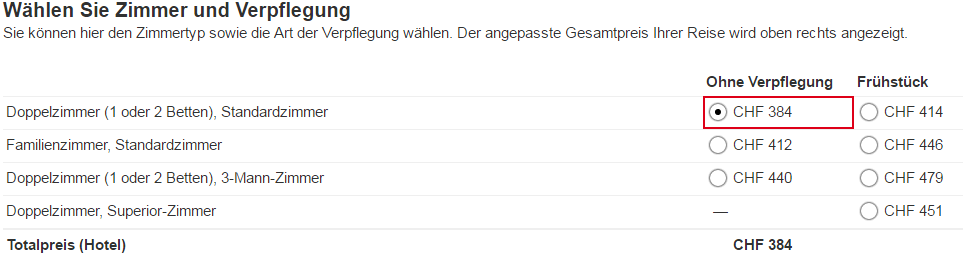
\includegraphics[width=0.8\textwidth]{images/travel-configuration.png}
	\caption{Hotelconfiguration von Hotel und Flug auf travel.ch}
	\label{fig:recherche:travelch:configuration}
\end{figure}
Auf der Konfigurationsseite des Hotels werden weitere Informationen wie Checkin-Daten, Hoteldetails, Detailierten Bewertungen, Hotelfacts, etc. angezeigt. Das wichtigste ist jedoch die oben dargestellte Matrix. Sie erlaubt dem Kunden das Hotelzimmer zu konfigurieren. Die Spalten der Matrix sind die Zimmer-, und die Kolonnen die Verpflegungstypen.

\begin{figure}[H]
	\centering
	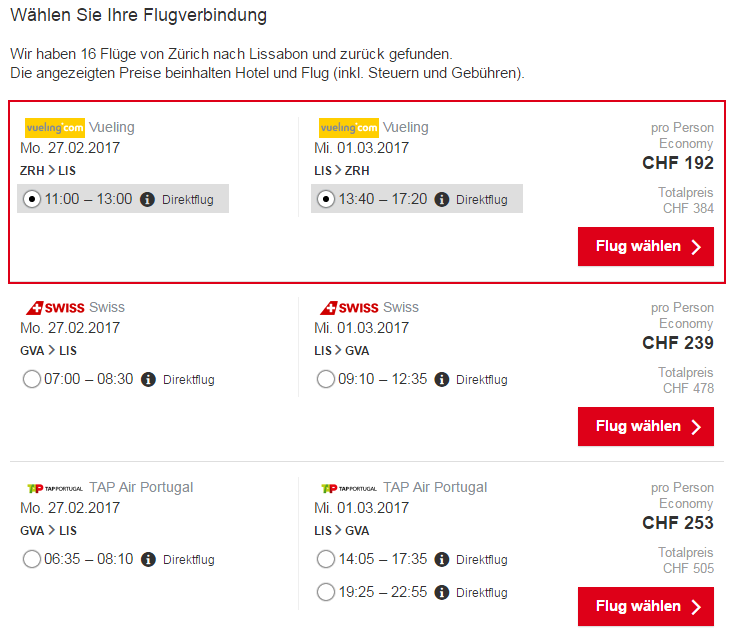
\includegraphics[width=0.8\textwidth]{images/travel-flights.png}
	\caption{Hotel und Flug Flugresultate auf travel.ch}
	\label{fig:recherche:travelch:flights}
\end{figure}
Zum Schluss wird dem Kunden noch eine Auswahl von Flügen angeboten.

Danach gelangt der User in den Checkout Prozess, wo er seine persönlichen Daten eingeben muss und die Zahlung tätigen kann. Dies wurde jedoch an ein externes System ausgelagert und kann deshalb nicht mehr im BPMN dargestellt werden, da es keine zugängliche API dafür gibt. 

\section{Programme}
In diesem Abschnitt werden verschiedene Programme vorgestellt und analysierten, ob sie für die Umsetzung dieses Projekte in Frage kommen. Dazu wird zuvor definiert, was die Anforderungen an das Programm sind.

\subsection{Anforderungen}
\label{sec:Recherche:programme:anforderungen}
Eine zentrale Eigenschaft des Programmes ist, dass es eine Process Engine enthält. Dieses ermöglicht es, ein Prozess nicht nur in dem Tool zu zeichnen, sondern diesen auch auszuführen. Gemäss Aufgabenstellung muss das Tool auch die Datentransformation mittels XSLT unterstützen.

In den Abschnitten \cref{sec:Recherche:rahmenbedingungen:prozesse} \nameref{sec:Recherche:rahmenbedingungen:prozesse} und \cref{sec:Recherche:rahmenbedingungen:api} \nameref{sec:Recherche:rahmenbedingungen:api} wurde zudem beschrieben, dass das Programm auf den Betriebsystemen Windows und Unix lauffähig sein muss, sowie die Unterstützung von \Gls{glos:json} basierten \Glspl{glos:api} beinhalten muss.

Zusätzlich sollte die Software gratis sein.

\subsection{Programmanalyse}
\label{sec:Recherche:programme:analyse}
Die folgende Tabelle vergleicht verschiedene BPMN Tools auf die zuvor definierten Anforderungen (siehe \cref{sec:Recherche:programme:anforderungen} \nameref{sec:Recherche:programme:anforderungen}).
\begin{table}[H] 
	\caption{Programme - Feature Gegenüberstellung}
	\centering
	\label{sec:Recherche:programme:programmanalyse}
	
	\begin{tabular}{ | c | c | c | c | c | c | } 
		\hline 
		\textbf{Programm} & \textbf{\begin{tabular}[x]{@{}c@{}}Process\\Engine\end{tabular}} & \textbf{\begin{tabular}[x]{@{}c@{}}Windows\\\& Linux\end{tabular}} & \textbf{\begin{tabular}[x]{@{}c@{}}API mittels\\JSON\end{tabular}} & \textbf{XSLT} & \textbf{Gratis} \\ \hline 
		Activiti\footcite{Activiti_2016-06-12} & x & x &  &  & x \\ \hline
		Yaoqiang\footcite{Yaoqiang_2016-06-12} &  & x &  &  &  \\ \hline
		jBPM\footcite{jBPM_2016-06-12} & x & x &  &  & x \\ \hline
		Imixs\footcite{Imixs_2016-06-12} & x & x &  &  & x \\ \hline
		\begin{tabular}[x]{@{}c@{}}IBM Business\\Process Manager\footcite{IBM_Business_Process_Manager_2016-06-12}\end{tabular} & x & & x &  &  \\ \hline
		Camuda\footcite{Camuda_2016-06-12} & x & x &  &  & x \\ \hline
		
		Drools\footcite{Drools_2016-06-12} & x & x &  &  & x \\ \hline
		Bonita\footcite{Bonitasoft_2016-06-12} & x & x & & x & x \\ \hline
		BizTalk\footcite{BizTalk_2016-06-12} & x &  & x & x &  \\ \hline		
	\end{tabular} 
\end{table}

Von den Funktionen ist Microsoft's BizTalk die geeignetste Variante. Jedoch läuft dieses Programm nicht auf Linux und es ist nicht gratis. Die zweitbeste Wahl ist Bonita von Bonitasoft, welches keine \Gls{glos:api} Anfragen mittels \Gls{glos:json} unterstützt.